% Copyright (c) 2012-2013 by the University of Waikato, Hamilton, NZ. 
% This work is made available under the terms of the 
% Creative Commons Attribution-ShareAlike 3.0 license, 
% http://creativecommons.org/licenses/by-sa/3.0/. 
%
% Version: $Revision$

\documentclass[a4paper]{book}

\usepackage{wrapfig}
\usepackage{graphicx}
\usepackage{hyperref}
\usepackage{multirow}
\usepackage{scalefnt}
\usepackage{tikz}

% watermark -- for draft stage
\usepackage[firstpage]{draftwatermark}
\SetWatermarkLightness{0.9}
\SetWatermarkScale{5}

% Copyright (c) 2009 by the University of Waikato, Hamilton, NZ. 
% This work is made available under the terms of the 
% Creative Commons Attribution-ShareAlike 3.0 license, 
% http://creativecommons.org/licenses/by-sa/3.0/. 
%
% Version: $Revision$

\newenvironment{tight_itemize}{
\begin{itemize}
  \setlength{\itemsep}{1pt}
  \setlength{\parskip}{0pt}
  \setlength{\parsep}{0pt}}{\end{itemize}
}

\newenvironment{tight_enumerate}{
\begin{enumerate}
  \setlength{\itemsep}{1pt}
  \setlength{\parskip}{0pt}
  \setlength{\parsep}{0pt}}{\end{enumerate}
}

% if you just need a simple heading
% Usage:
%   \heading{the text of the heading}
\newcommand{\heading}[1]{
  \vspace{0.3cm} \noindent \textbf{#1} \newline
}

\newcommand{\icon}[1]{\tikz[baseline=-3pt]\node[inner sep=0pt,outer sep=0pt]{\includegraphics[height=1.1em]{#1}};}


\title{
  \textbf{ADAMS} \\
  {\Large \textbf{A}dvanced \textbf{D}ata mining \textbf{A}nd \textbf{M}achine
  learning \textbf{S}ystem} \\
  {\Large Module: adams-pdf} \\
  \vspace{1cm}
  
\includegraphics[width=2cm]{images/pdf-module.png} \\
}
\author{
  Peter Reutemann
}

\setcounter{secnumdepth}{3}
\setcounter{tocdepth}{3}

\begin{document}

\begin{titlepage}
\maketitle

\thispagestyle{empty}
\center
\begin{table}[b]
	\begin{tabular}{c l l}
		\parbox[c][2cm]{2cm}{\copyright 2012-2013} &
		\parbox[c][2cm]{5cm}{
\includegraphics[width=5cm]{images/coat_of_arms.pdf}} \\
	\end{tabular}
	
\includegraphics[width=12cm]{images/cc.png} \\
\end{table}

\end{titlepage}

\tableofcontents
\listoffigures
%\listoftables

%%%%%%%%%%%%%%%%%%%%%%%%%%%%%%%%%%%
\chapter{Introduction}
The \textit{pdf} module adds PDF authoring capabilities to ADAMS. 
This is possible thanks to the iText \cite{itext} and jPod Renderer \cite{jpod} 
libraries for creating, manipulating and viewing of PDF files.

%%%%%%%%%%%%%%%%%%%%%%%%%%%%%%%%%%%
\chapter{Flow}
For manipulating and viewing PDF files, you can use the following actors:
\begin{tight_itemize}
	\item \textit{PDFCreate} -- for creating PDFs, using text files, 
	spreadsheets and images.\footnote{adams-pdf-create\_pdf.flow}
	\item \textit{PDFExtract} -- extracts a range of pages.
	\item \textit{PDFExtractImages} -- extracts the images from a PDF.\footnote{adams-pdf-extract\_images.flow}
	\item \textit{PDFExtractText} -- obtaining the plain text of the PDF.\footnote{adams-pdf-extract\_text.flow}
	\item \textit{PDFMerge} -- merges several PDFs into a single one.\footnote{adams-pdf-page\_count.flow}
	\item \textit{PDFPageCount} -- determines the number of pages in a 
	PDF.\footnote{adams-pdf-page\_count.flow}
	\item \textit{PDFViewer} -- for viewing PDFs.\footnote{adams-pdf-view\_pdf.flow}
\end{tight_itemize}

\heading{Creating PDFs}
Generating a PDF using the \textit{PDFCreate} transformer is really easy.
The transformer takes an array of file names as input, which will all get added
to the specified output PDF file. Basic options, like page size and orientation,
can be set as well. How and what files get added to the PDF, is determined by
the ``proclets'', i.e., little processor classes, that you specify and configure:
\begin{tight_itemize}
	\item \textit{CsvPdfProclet} -- for adding CSV files as tables.
	\item \textit{HeadlinePdfProclet} -- for adding a headline.
	\item \textit{ImagePdfProclet} -- for adding images (GIF, JPEG, PNG).
	\item \textit{PlainTextPdfProclet} -- for adding plain text files as paragraphs.
\end{tight_itemize}

Figure \ref{pdf-create-flow} shows a flow\footnote{adams-pdf-create\_pdf.flow} 
that adds all files (i.e., three) found in a directory to a single PDF. 
Figures \ref{pdf-create-output1}, \ref{pdf-create-output2} and 
\ref{pdf-create-output3} show the resulting pages of the PDF in the viewer.

\begin{figure}[htb]
  \centering
  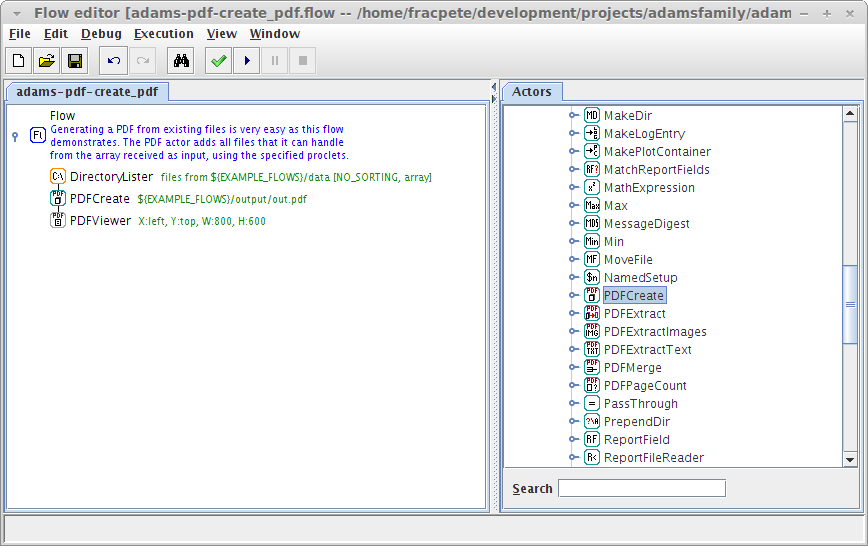
\includegraphics[width=10.0cm]{images/pdf-create-flow.png}
  \caption{Flow for creating a PDF file from various sources.}
  \label{pdf-create-flow}
\end{figure}

\begin{figure}[htb]
  \centering
  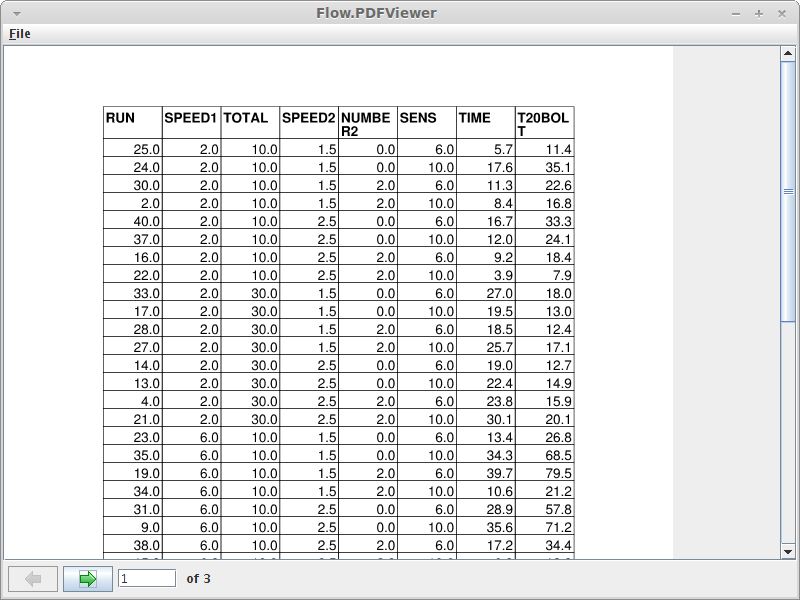
\includegraphics[width=10.0cm]{images/pdf-create-output1.png}
  \caption{CSV files get added as tables.}
  \label{pdf-create-output1}
\end{figure}

\begin{figure}[htb]
  \centering
  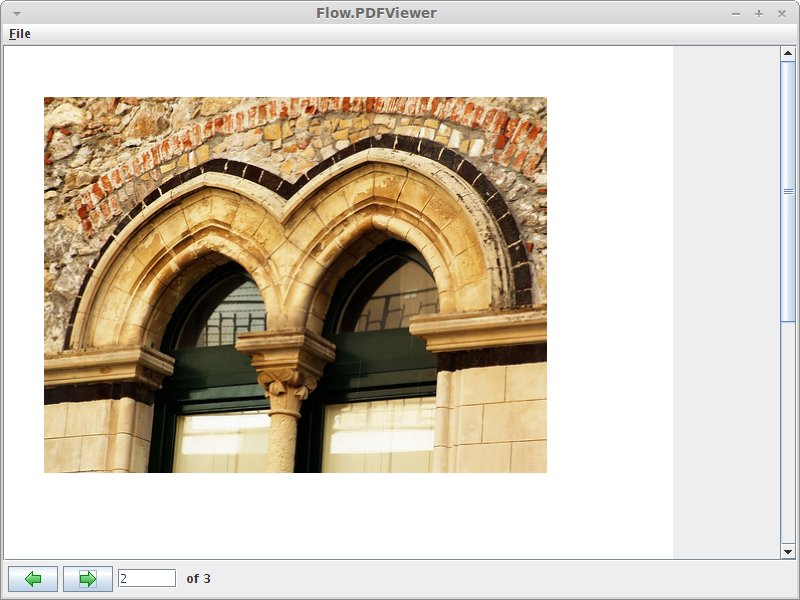
\includegraphics[width=10.0cm]{images/pdf-create-output2.png}
  \caption{Images can get inserted as well.}
  \label{pdf-create-output2}
\end{figure}

\begin{figure}[htb]
  \centering
  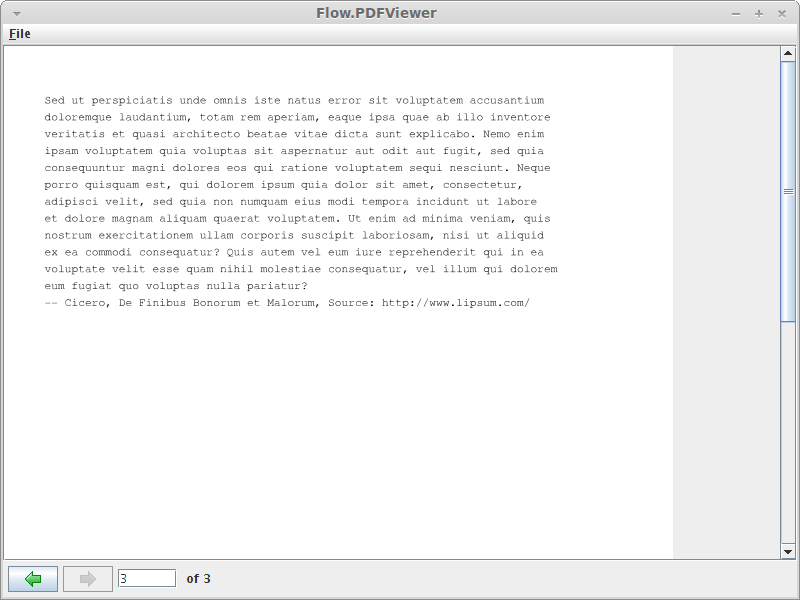
\includegraphics[width=10.0cm]{images/pdf-create-output3.png}
  \caption{Plain text files get added as simple text.}
  \label{pdf-create-output3}
\end{figure}

%%%%%%%%%%%%%%%%%%%%%%%%%%%%%%%%%%%
\chapter{Tools}
The \textit{PDF viewer} can be used to load and browse PDF files. Figure 
\ref{pdf-viewer} shows a screenshot of the viewer with a PDF file loaded.

\begin{figure}[htb]
  \centering
  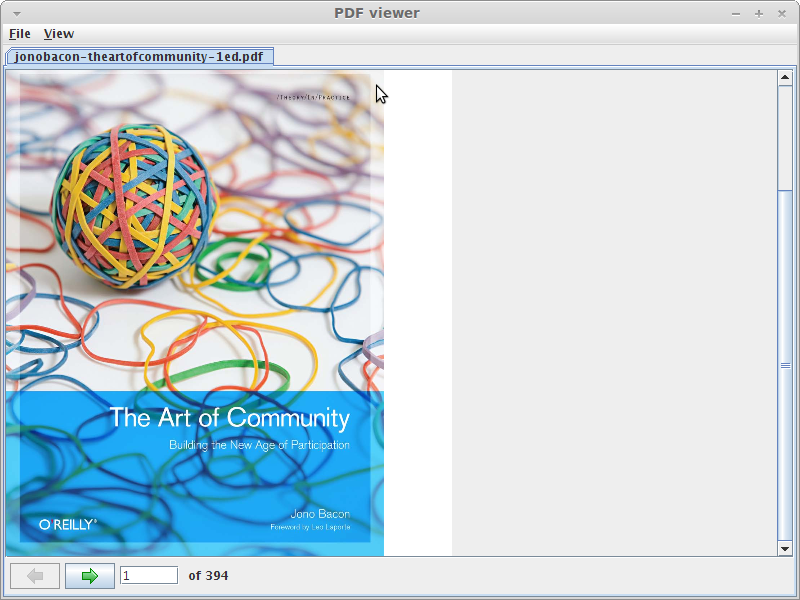
\includegraphics[width=10.0cm]{images/pdf-viewer.png}
  \caption{Viewer for PDF files.}
  \label{pdf-viewer}
\end{figure}

%%%%%%%%%%%%%%%%%%%%%%%%%%%%%%%%%%%
\chapter{Troubleshooting}
\begin{tight_itemize}
	\item \textbf{Problem:} 64bit Linux shows error message when viewing PDF 
	that `libfreetype.so' library was not found (``UnsatisfiedLinkError"). \\
	\textbf{Solution:} Make sure that /usr/lib/libfreetype.so exists. If not, 
	add a symbolic link to the 64bit library, using a similar command as 
	follows (for Kubuntu 11.10 or LinuxMint 11, 13):
\begin{verbatim}
  sudo ln -s /usr/lib/x86_64-linux-gnu/libfreetype.so.6 /usr/lib/libfreetype.so
\end{verbatim}
    And restart the application.
\end{tight_itemize}

%%%%%%%%%%%%%%%%%%%%%%%%%%%%%%%%%%%
% Copyright (c) 2009-2012 by the University of Waikato, Hamilton, NZ. 
% This work is made available under the terms of the 
% Creative Commons Attribution-ShareAlike 4.0 license,
% http://creativecommons.org/licenses/by-sa/4.0/.
%
% Version: $Revision$

\begin{thebibliography}{999}
	% to make the bibliography appear in the TOC
	\addcontentsline{toc}{chapter}{Bibliography}

    % references
	\bibitem{adams}
		\textit{ADAMS} -- Advanced Data mining and Machine learning System \\
		\url{https://adams.cms.waikato.ac.nz/}{}

	\bibitem{esrigrid}
	 	\textit{Esri Grid} -- a raster GIS file format deveoped by Esri. \\
		\url{https://en.wikipedia.org/wiki/Esri\_grid}{}

	\bibitem{kml}
	 	\textit{Keyhole Markup Language} -- an XML notation for expressing
	 	geographic annotation and visualization within Internet-based,
	 	two-dimensional maps and three-dimensional Earth browsers. \\
		\url{http://en.wikipedia.org/wiki/Keyhole\_Markup\_Language}{}

	\bibitem{postgresql}
	 	\textit{PostgreSQL} -- a powerful, open source object-relational
	 	database system. \\
		\url{http://www.postgresql.org/}{}

	\bibitem{postgis}
		\textit{PostGIS} -- a spatial database extender for PostgreSQL
		object-relational database. It adds support for geographic
		objects allowing location queries to be run in SQL.  \\
		\url{http://postgis.net/}{}

	\bibitem{srid4269}
	 	\textit{SRID 4269} -- or NAD 83 (North American Datum). \\
		\url{http://spatialreference.org/ref/epsg/4269/}{}

	\bibitem{mysql}
		\textit{MySQL} -- an open-source relational database management
		system (RDBMS) \\
		\url{http://www.mysql.com/}{}

\end{thebibliography}


\end{document}
